\chapter{Preparación del entorno de la máquina virtual}

Partiremos de la máquina virtual proporcionada por el profesor, la cual tiene instalado el sistema operativo Ubuntu 22.04.3 LTS.

\section{Preparación de Cassandra}

Primero instalaremos Cassandra, para ello primero actualizaremos el sistema operativo. El comando \texttt{sudo apt update} actualiza la lista de paquetes disponibles y sus versiones, mientras que el comando \texttt{sudo apt upgrade} instala las actualizaciones disponibles.

\begin{lstlisting}[language=bash]
sudo apt update && sudo apt upgrade
\end{lstlisting}

\begin{figure}[H]
    \centering
    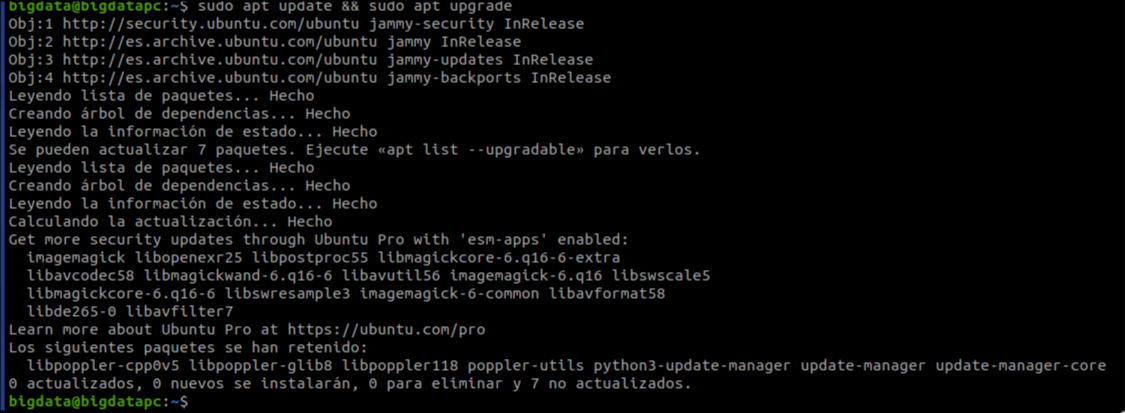
\includegraphics[width=0.8\textwidth]{figures/1.png}
    \caption{Actualización del sistema operativo}
\end{figure}

Ahora instalaremos Python 2, ya que Cassandra requiere esta versión de Python. Para ello, ejecutamos el siguiente comando:

\begin{lstlisting}[language=bash]
sudo apt install python2
\end{lstlisting}

\begin{figure}[H]
    \centering
    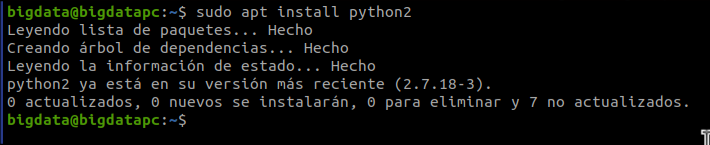
\includegraphics[width=0.8\textwidth]{figures/2.png}
    \caption{Instalación de Python 2}
\end{figure}

Después, descargaremos el archivo .tar.gz de Cassandra desde la página oficial de Apache. Para ello, ejecutamos el siguiente comando:

\begin{lstlisting}[language=bash]
    wget https://dlcdn.apache.org/cassandra/3.11.16/apache-cassandra-3.11.16-bin.tar.gz
\end{lstlisting}

\begin{figure}[H]
    \centering
    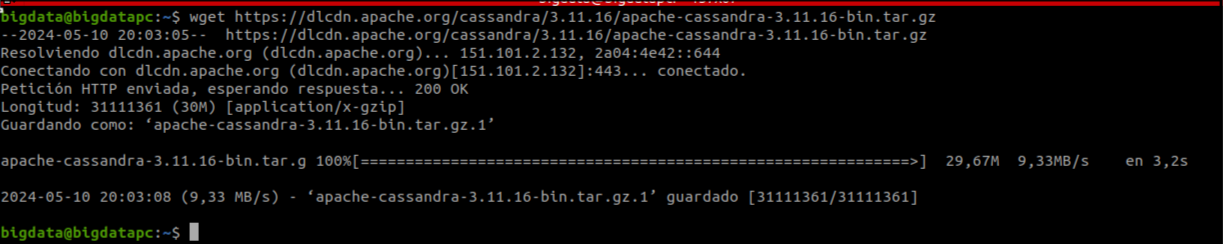
\includegraphics[width=0.8\textwidth]{figures/3.png}
    \caption{Descarga de Cassandra}
\end{figure}

Descomprimimos el archivo .tar.gz con el siguiente comando:

\begin{lstlisting}[language=bash]
    tar -xvzf apache-cassandra-3.11.16-bin.tar.gz
\end{lstlisting}

\begin{figure}[H]
    \centering
    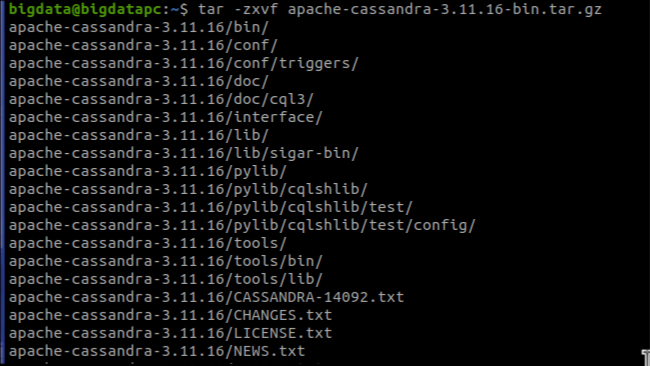
\includegraphics[width=0.8\textwidth]{figures/4.png}
    \caption{Descompresión de Cassandra}
\end{figure}

Por último, eliminamos el archivo .tar.gz con el siguiente comando:

\begin{lstlisting}[language=bash]
    rm apache-cassandra-3.11.16-bin.tar.gz
\end{lstlisting}

\begin{figure}[H]
    \centering
    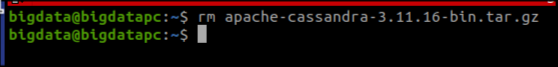
\includegraphics[width=0.8\textwidth]{figures/5.png}
    \caption{Eliminación del archivo .tar.gz}
\end{figure}

\section{Desplegar HDFS}

HDFS ya está instalado por defecto en la máquina virtual en la carpeta \texttt{~/hadoop-3.3.6}. Para desplegar HDFS ejecutamos el siguiente comando:

\begin{lstlisting}[language=bash]
    ~/hadoop-3.3.6/sbin/start-dfs.sh
\end{lstlisting}

\begin{figure}[H]
    \centering
    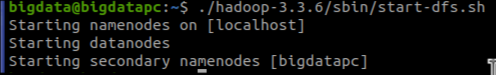
\includegraphics[width=0.8\textwidth]{figures/6.png}
    \caption{Despliegue de HDFS}
\end{figure}

Ahora para comprobar que HDFS se ha desplegado correctamente, ejecutamos el siguiente comando:

\begin{lstlisting}[language=bash]
    jps
\end{lstlisting}

\begin{figure}[H]
    \centering
    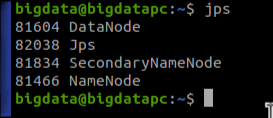
\includegraphics[width=0.8\textwidth]{figures/7.png}
    \caption{Comprobación de HDFS}
\end{figure}

Ahora ya podemos ejecutar comandos de HDFS, como por ejemplo el siguiente comando que muestra los archivos en el sistema de archivos HDFS:

\begin{lstlisting}[language=bash]
    ~/hadoop-3.3.6/bin/hdfs dfs -ls /
\end{lstlisting}

\begin{figure}[H]
    \centering
    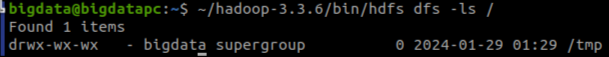
\includegraphics[width=0.8\textwidth]{figures/8.png}
    \caption{Comando de HDFS}
\end{figure}

\section{Desplegar PostgreSQL}

Postgres también está instalado por defecto en la máquina virtual, además se arranca por defecto al iniciar la sesión en la máquina virtual. El motivo por el que arranca por defecto es que se ha configurado como un servicio de systemd, por lo que se inicia automáticamente al arrancar el sistema.

Para comprobar que Postgres se ha desplegado correctamente, ejecutamos el siguiente comando:

\begin{lstlisting}[language=bash]
    sudo systemctl status postgresql
\end{lstlisting}

\begin{figure}[H]
    \centering
    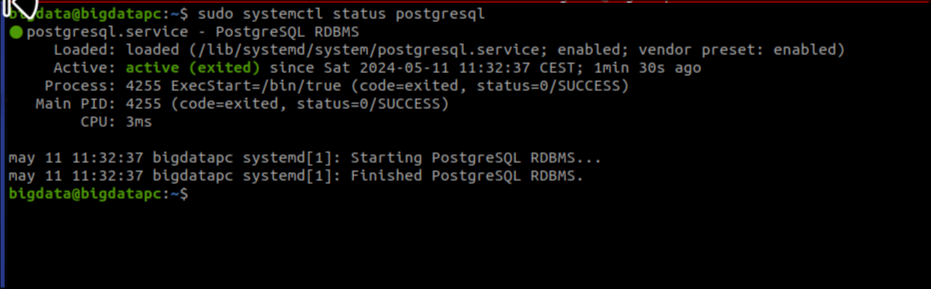
\includegraphics[width=0.8\textwidth]{figures/9.png}
    \caption{Comprobación de Postgres}
\end{figure}

Ahora para asegurarnos de que todo funciona correctamente, nos conectamos a la consola de Postgres y ejecutamos un comando de prueba. Para ello, ejecutamos el siguiente comando:

\begin{lstlisting}[language=bash]
    sudo -u postgres psql
\end{lstlisting}

\begin{lstlisting}[language=sql]
    SELECT version();
\end{lstlisting}

\begin{figure}[H]
    \centering
    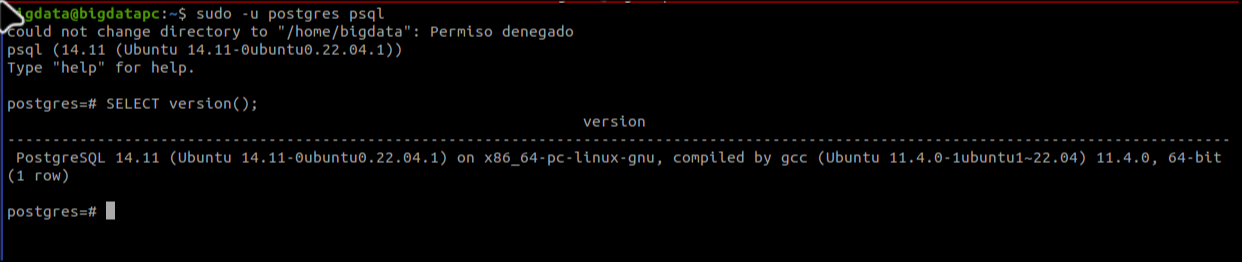
\includegraphics[width=0.8\textwidth]{figures/10.png}
    \caption{Comando de prueba de Postgres}
\end{figure}

\section{Desplegar Cassandra}

Primero nos moveremos a la carpeta de Cassandra con el siguiente comando:

\begin{lstlisting}[language=bash]
    cd ~/apache-cassandra-3.11.16
\end{lstlisting}

Acto seguido, arrancamos el servicio de Cassandra con el siguiente comando:

\begin{lstlisting}[language=bash]
    bin/cassandra
\end{lstlisting}

\begin{figure}[H]
    \centering
    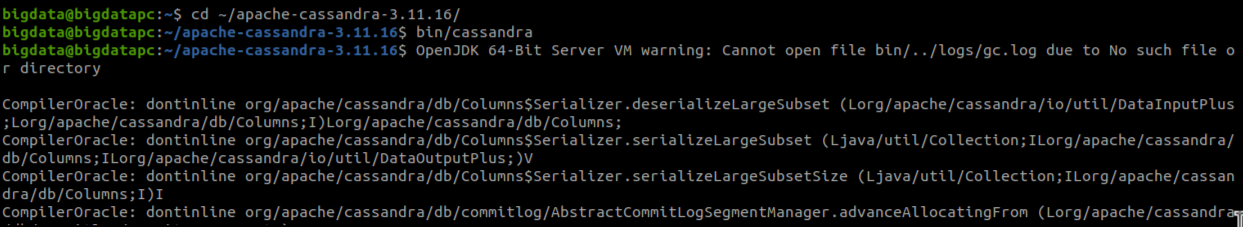
\includegraphics[width=0.8\textwidth]{figures/11.png}
    \caption{Despliegue de Cassandra}
\end{figure}

Ahora inciamos la consola de Cassandra con el siguiente comando:

\begin{lstlisting}[language=bash]
    bin/cqlsh
\end{lstlisting}

\begin{figure}[H]
    \centering
    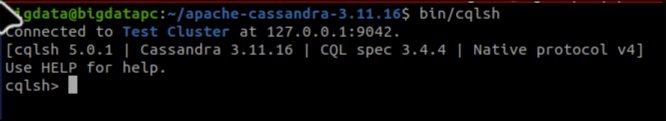
\includegraphics[width=0.8\textwidth]{figures/12.png}
    \caption{Consola de Cassandra}
\end{figure}

Por último, tendremos que generar un keyspace que nos servirá más adelante.

\begin{lstlisting}[language=sql]
    CREATE KEYSPACE IF NOT EXISTS practica WITH REPLICATION = {'class': 'SimpleStrategy', 'replication_factor': 1};
\end{lstlisting}

Salimos de la consola de Cassandra con el siguiente comando:

\begin{lstlisting}[language=sql]
    exit
\end{lstlisting}

\begin{figure}[H]
    \centering
    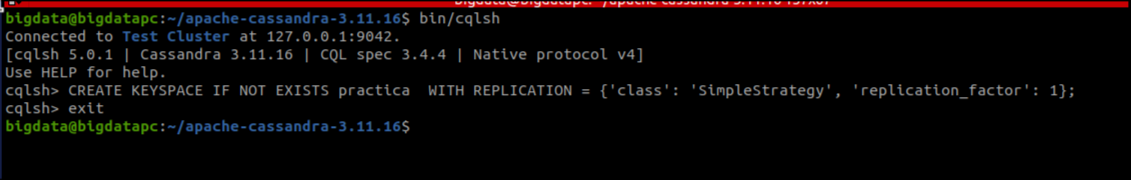
\includegraphics[width=0.8\textwidth]{figures/13.png}
    \caption{Creación de keyspace en Cassandra}
\end{figure}

\section{Desplegar clúster de Spark Standalone}

Vamos a ver como configurar y arrancar un despliegue de 1 nodo Master y 2 nodos Worker de Spark Standalone.

Primero, nos movemos a la carpeta de Spark con el siguiente comando:

\begin{lstlisting}[language=bash]
    cd ~/spark-3.3.3-bin-hadoop3
\end{lstlisting}

\begin{figure}[H]
    \centering
    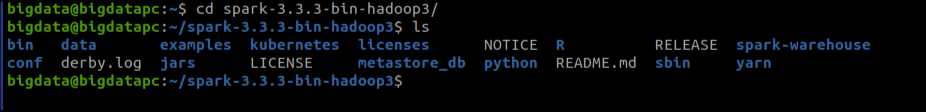
\includegraphics[width=0.8\textwidth]{figures/14.png}
    \caption{Cambio de directorio a Spark}
\end{figure}

Una vez que estamos en la carpeta de Spark, arrancamos el Master con el siguiente comando:

\begin{lstlisting}[language=bash]
    sbin/start-master.sh
\end{lstlisting}

\begin{figure}[H]
    \centering
    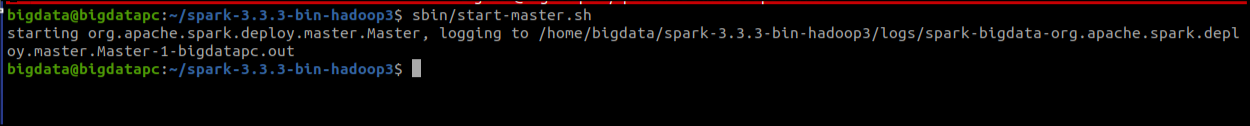
\includegraphics[width=0.8\textwidth]{figures/15.png}
    \caption{Arranque del Master de Spark}
\end{figure}

En la ejecución del comando anterior, se nos muestra el archivo de los logs del Master, en este caso el archivo es \textit{/home/bigdata/spark-3.3.3-bin-hadoop3/logs/spark-bigdata-org.apache.spark.deploy.master.Master-1-bigdatac.out}. Con un par de comandos sacaremos la URL del Master, que es la dirección que usaremos para conectarnos a la interfaz web del Master.

\begin{lstlisting}[language=bash]
    cat /home/bigdata/spark-3.3.3-bin-hadoop3/logs/spark-bigdata-org.apache.spark.deploy.master.Master-1-bigdatac.out | grep 'http://' | awk '{print $NF}'
\end{lstlisting}

\begin{figure}[H]
    \centering
    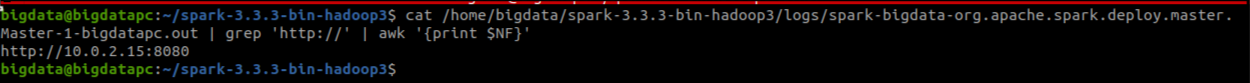
\includegraphics[width=0.8\textwidth]{figures/16.png}
    \caption{URL del Master de Spark}
\end{figure}

En nuestro caso, si nos conectamos a la URL \texttt{http://10.0.2.15:8080/} podremos ver la interfaz web del Master de Spark.

\begin{figure}[H]
    \centering
    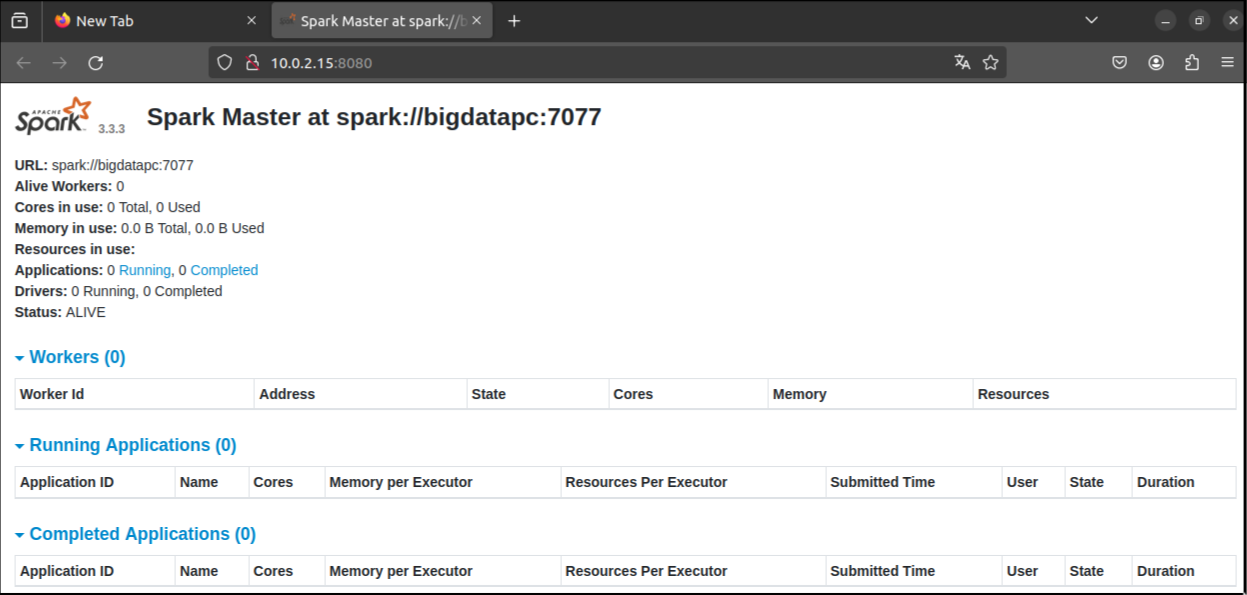
\includegraphics[width=0.8\textwidth]{figures/17.png}
    \caption{Interfaz web del Master de Spark}
\end{figure}

Para los workes, también necesitaremos una URL que encontraremos en los logs del Master. Para ello, ejecutamos el siguiente comando:

\begin{lstlisting}[language=bash]
    cat /home/bigdata/spark-3.3.3-bin-hadoop3/logs/spark-bigdata-org.apache.spark.deploy.master.Master-1-bigdatac.out | grep 'spark://' | awk '{print $NF}'
\end{lstlisting}

\begin{figure}[H]
    \centering
    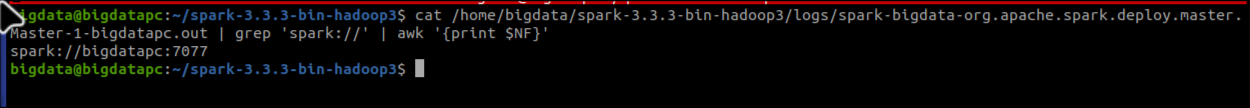
\includegraphics[width=0.8\textwidth]{figures/18.png}
    \caption{URL de los Workers de Spark}
\end{figure}

Antes de desplegar los Workres, para poder tener dos Workers en una misma máquina vamos a modificar la configuración del archivo \texttt{conf/spark-env.sh}. Para ello, ejecutamos el siguiente comando:

\begin{lstlisting}[language=bash]
    vim conf/spark-env.sh
\end{lstlisting}

Y añadimos las 3 siguientes líneas al final del archivo:

\begin{lstlisting}[language=bash]
    SPARK_WORKER_INSTANCES=2
    SPARK_WORKER_CORES=2
    SPARK_WORKER_MEMORY=1g
\end{lstlisting}

\begin{figure}[H]
    \centering
    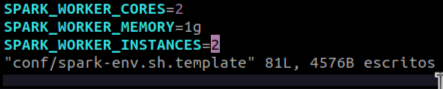
\includegraphics[width=0.8\textwidth]{figures/20.png}
    \caption{Configuración de los Workers de Spark}
\end{figure}

Ahora arrancaremos dos Workers con 1GB de memoria y 2 cores (la configuración que hemos especificado). Es necesario especificar la memoria y los cores ya que por defecto los Workers usarán toda la memoria y todos los cores disponibles.

\begin{lstlisting}[language=bash]
    sbin/start-slave.sh spark://bigdatapc:7077
\end{lstlisting}

\begin{figure}[H]
    \centering
    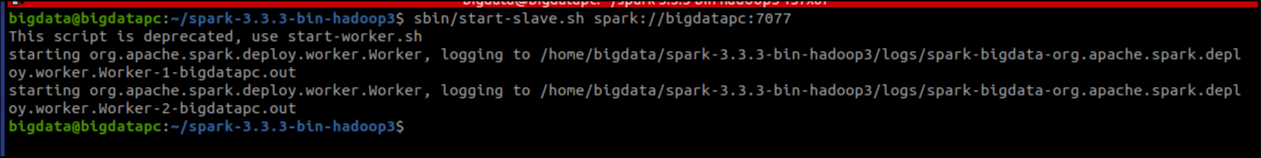
\includegraphics[width=0.8\textwidth]{figures/19.png}
    \caption{Arranque de los Workers de Spark}
\end{figure}

Si nos vamos a la interfaz web del Master de Spark, podremos ver los Workers conectados. En esta interfaz se nos muestra el id del nodo Worker, la dirección IP, el número de cores, la memoria disponible, la carga de trabajo, la memoria utilizada y el estado del nodo. Además, arriba se nos muestra un resumen de todos los recursos usados y de las aplicaciones en ejecución.

\begin{figure}[H]
    \centering
    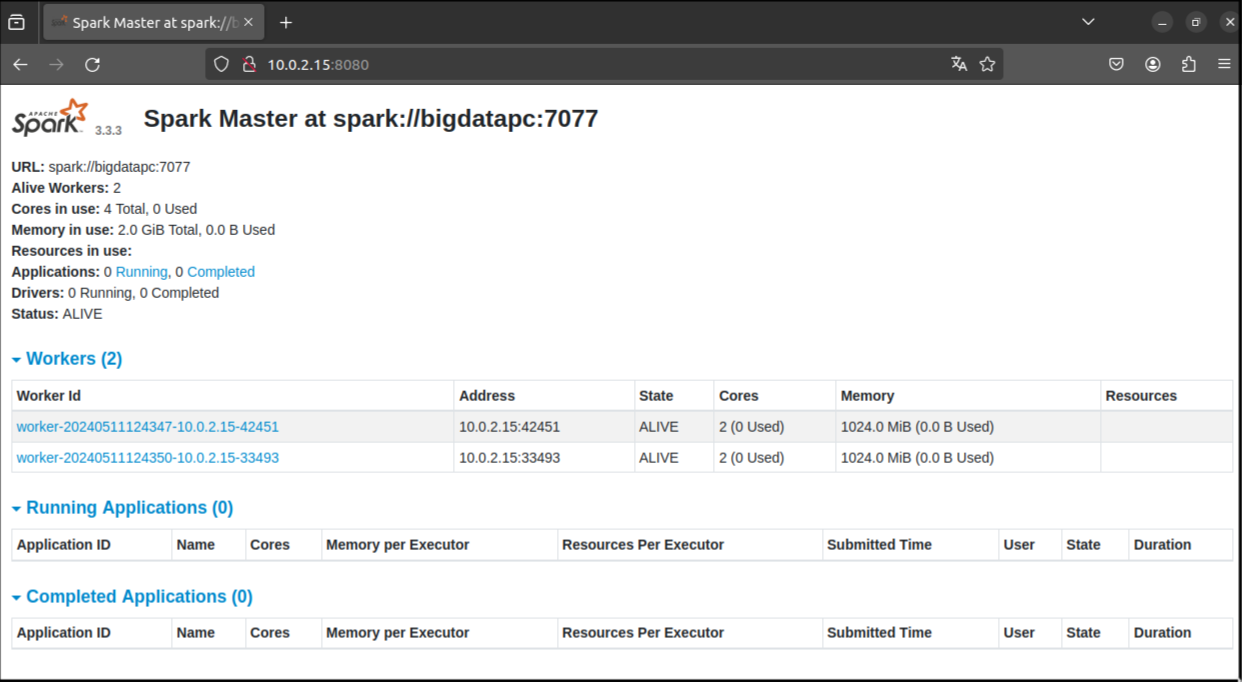
\includegraphics[width=0.8\textwidth]{figures/21.png}
    \caption{Interfaz web del Master de Spark con los Workers conectados}
\end{figure}

\section{Desplegar una shell de Spark}

El primer paso será descargar los conectores de Postgres y Cassandra. Primero nos moveremos a la carpeta \textit{spark-3.3.3-bin-hadoop3/jars} y a continuación descargaremos los conectores con los siguientes comandos:

\begin{lstlisting}[language=bash]
    cd ~/spark-3.3.3-bin-hadoop3/jars
    wget https://jdbc.postgresql.org/download/postgresql-42.7.3.jar
    wget https://repo1.maven.org/maven2/com/datastax/spark/spark-cassandra-connector_2.12/3.3.0/spark-cassandra-connector_2.12-3.3.0.jar
\end{lstlisting}

\begin{figure}[H]
    \centering
    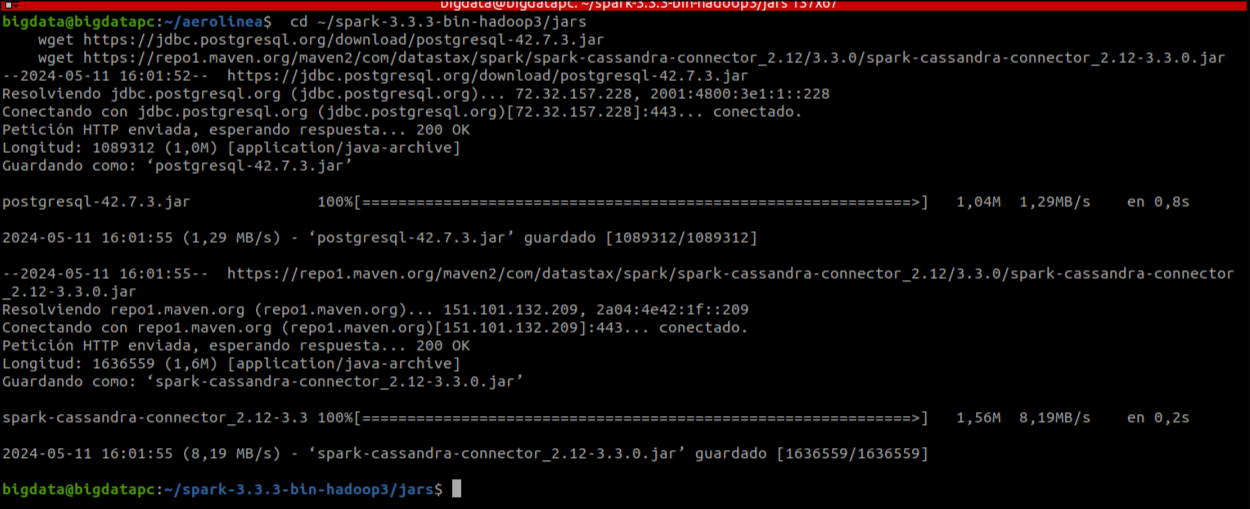
\includegraphics[width=0.8\textwidth]{figures/22.png}
    \caption{Descarga de los conectores de Postgres y Cassandra}
\end{figure}

Ahora, para arrancar una shell de Spark, ejecutaremos el siguiente comando. En este comando especificamos la memoria que queremos que use el driver y los executors, así como el número de cores que queremos que use el driver y los executors. Además, especificamos los conectores que hemos descargado anteriormente.

\begin{lstlisting}[language=bash]
bin/spark-shell --master spark://bigdatapc:7077 --driver-memory 1G --executor-memory 1G --total-executor-cores 2 --executor-cores 2 --jars jars/postgresql-42.7.3.jar,jars/spark-cassandra-connector_2.12-3.3.0.jar
\end{lstlisting}

\begin{figure}[H]
    \centering
    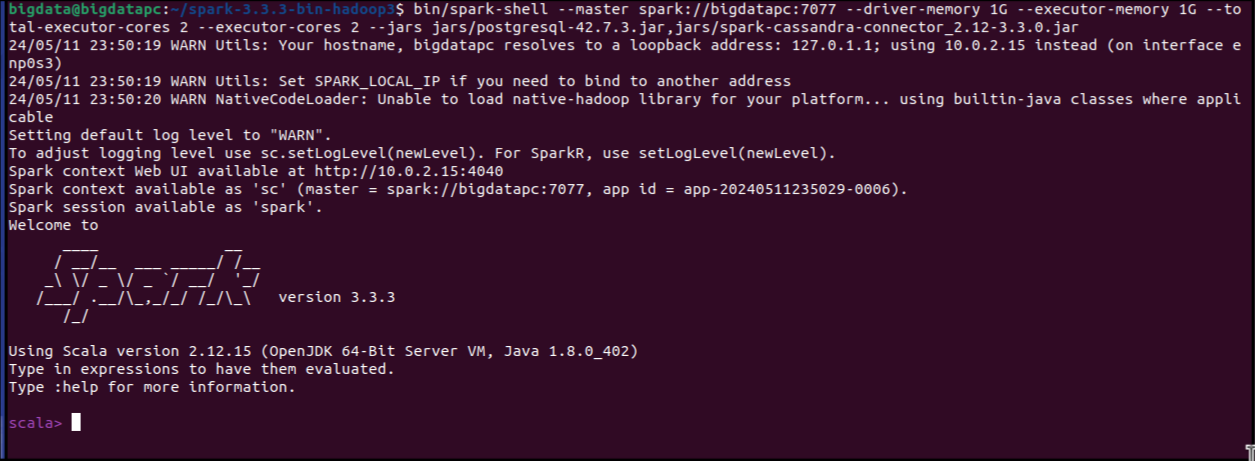
\includegraphics[width=0.8\textwidth]{figures/23.png}
    \caption{Arranque de la shell de Spark}
\end{figure}

Si vamos a la web, veremos que se ha creado una aplicación en la interfaz web del Master de Spark.

\begin{figure}[H]
    \centering
    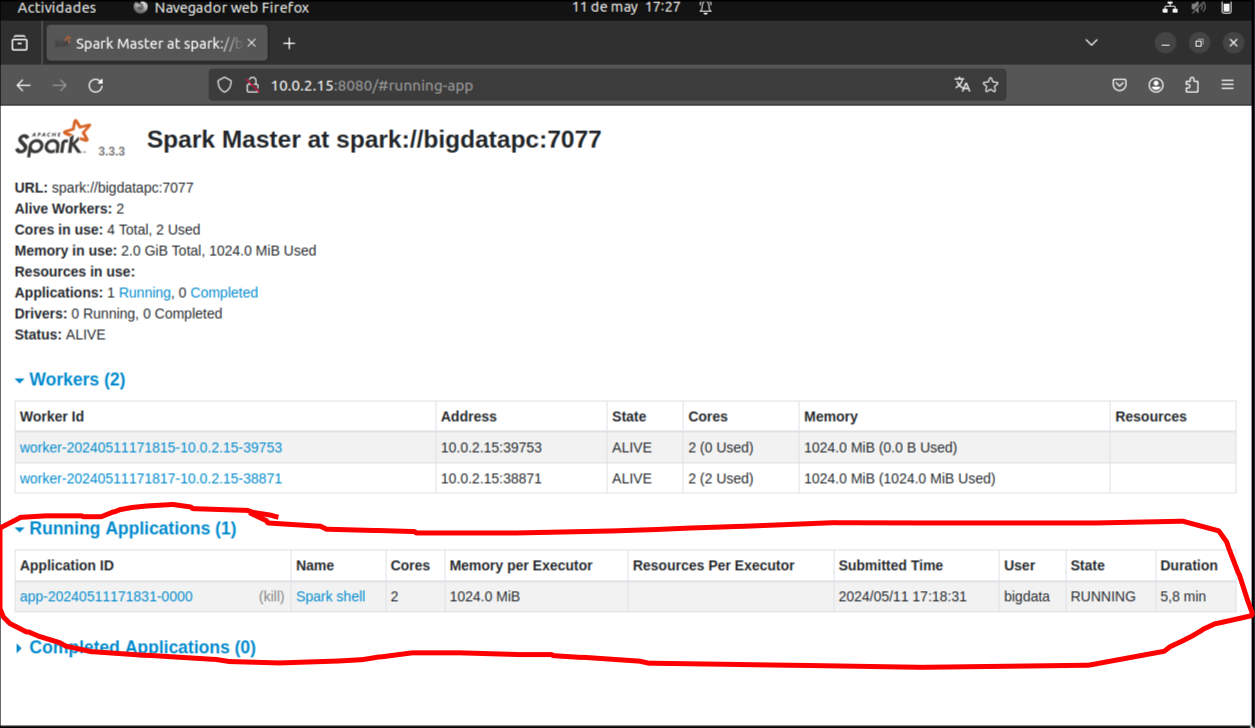
\includegraphics[width=0.8\textwidth]{figures/24.png}
    \caption{Interfaz web del Master de Spark con la aplicación creada}
\end{figure}

También, al arrancar la shell de Spark, se nos muestra la URL de la interfaz web de la shell de Spark:

\begin{figure}[H]
    \centering
    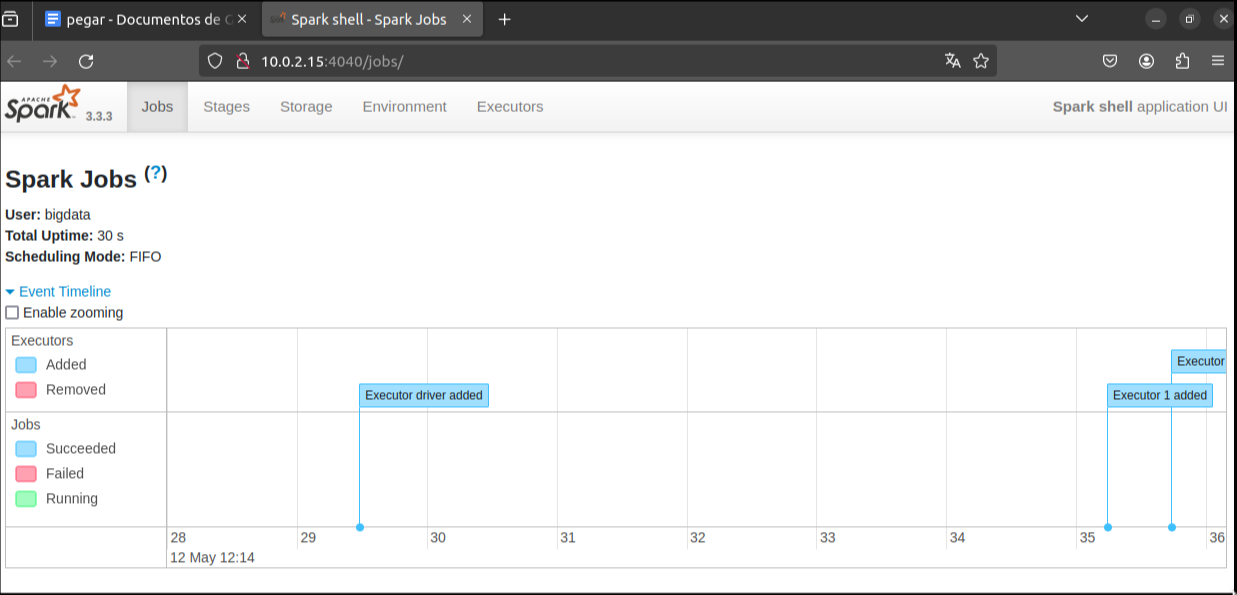
\includegraphics[width=0.8\textwidth]{figures/58.png}
    \caption{Interfaz web de la shell de Spark}
\end{figure}
